\begin{savequote}[75mm]
The real voyage of discovery consists not in seeking new landscapes, but in having new eyes.
\qauthor{Marcel Proust}
\end{savequote}

\chapter{The discovery of the Higgs boson and the role of the $H\rightarrow WW^{*}\rightarrow \ell\nu\ell\nu$ channel}

\section{Introduction}

This chapter presents the results of the search for the Higgs boson in $4.8 \ifb$ collected at $\sqrt{s} = 7 \TeV$ and $5.8 \ifb$ at $\sqrt{s} = 8 \TeV$. The results of three searches at $\sqrt{s} = 8 \TeV$ in the $H\to \gamma \gamma$, $H\to ZZ \to 4\ell$, and \HWWfull channels are combined with results of searches at $\sqrt{s} = 7 \TeV$ in the same search channels (as well as the $H\to\tau\tau$ production and associated production searches for $H\to b\bar{b}$). The results of this combination are a $5.9 \sigma$ detection of a new particle consistent with a Higgs boson. Rather than going into detail for all of the different Higgs decay searches, this chapter will discuss the three most sensitive channels and in particular give a comparison of the $\gamma\gamma$ and $4\ell$ channels to the $\ell\nu\ell\nu$ channel. This chapter is a summary of results presented in the ATLAS Higgs discovery publication\cite{Discovery}.


\section{Data and simulation samples}

The data sample used for the following results was taken in 2011 and 2012 at center of mass energies of $7$ and $8 \TeV$, respectively, with $4.8 \ifb$ collected at $7 \TeV$ and $5.8 \ifb$ collected at $8 \TeV$. Higgs production in the gluon fusion and vector boson fusion modes is modeled with \POWHEG for the hard scattering event and \PYTHIA for the showing and hadronization. Associated production of a Higgs with a vector boson or top quarks is modeled via \PYTHIA. 

Table~\ref{tab:disc_mc} shows the Monte Carlo generators used for modeling the signal and background processes relevant for the three analyses to be discussed. 

\begin{table}[h!]
\centering
\captionsetup{justification=centering}

%\begin{tabular*}{0.480\textwidth}{p{0.075\textwidth} p{0.180\textwidth} l}
\hspace{-10pt}
\begin{tabular}{|c|c|}
\hline
Process & Generator \\ \hline
ggF, VBF $H$ & \POWHEG + \PYTHIA \\ \hline
$WH$, $ZH$, $t\bar{t}H$ & \PYTHIA \\ \hline
$W$+jets, $\ZDY$ + jets & \ALPGEN + \HERWIG \\ \hline
$t\bar{t}$, $tW$, $tb$ & \MCATNLO + \HERWIG \\ \hline
$tqb$ & \ACERMC + \PYTHIA \\ \hline
$q\bar{q} \to WW$ & \MCATNLO + \HERWIG \\ \hline
$gg \to WW$ & \GGTOWW + \HERWIG \\ \hline
$q\bar{q} \to ZZ$ & \POWHEG + \PYTHIA \\ \hline
$gg \to ZZ$ & \GGTOZZ + \HERWIG \\ \hline
$WZ$ & \MADGRAPH + \PYTHIA, \HERWIG \\ \hline
$W\gamma$ + jets & \ALPGEN + \HERWIG \\ \hline
$W\gamma^*$ & \MADGRAPH + \PYTHIA \\ \hline
$q\bar{q}/gg \to \gamma \gamma$ & \SHERPA \\ \hline

\end{tabular}

\caption{
Monte carlo generators used to model signal and background for the Higgs search\cite{Discovery}.
}
\label{tab:disc_mc}
\end{table} 

\section{$H\to\gamma\gamma$ search}

The $H\to\gamma\gamma$ search is in essence a search for a peaked excess above the falling SM diphoton mass spectrum, with $m_{\gamma\gamma}$ as the ultimate discriminating variable. Events are selected by requiring two isolated photons, with the leading (sub-leading) photon required to have $E_{T} > 40 (30) \GeV$. In the $8 \TeV$ data, the photons are required to pass cut-based identification criteria consistent with a photon in the electromagnetic calorimeter and little leakage in the hadronic calorimeter. The main challenges for this analysis are accurate mass reconstruction and background estimation. These are the issues that will be discussed in this section.

\subsection{Diphoton invariant mass reconstruction}

In order to accurately reconstruct the invariant mass of the di-photon system, both the energy and direction of the photons must be measured well. The $\eta$ coordinate of the photons is calculated using the position of the primary vertex identified in the event as well as the entry points of the photons in the calorimeter. Therefore, the identification of hte primary vertex of the hard interaction is particularly important, and is done using a likelihood which combines the flight direction of the photons, the beam position measurement, and the scalar sum of $p_{T}^2$ for tracks at the primary vertex. This give a resolution of $15$ $\rm mm$ on the $z$ position of the primary vertex (which improves to $6$ $\rm mm$ for photons which convert to electron-positron pairs in the ID material). 

In the inclusive sample, there are $35251$ events observed in the $8 \TeV$ sample and $23788$ observed in the $7 \TeV$ sample. The total expected number of events for a Higgs at $126.5 \GeV$ is $110.5$ at $8 \TeV$ and $79.6$ at $7 \TeV$. The full width at half maximum (FWHM) of the mass distribution at this mass is $3.9 \GeV$ in the inclusive sample. The mass distribution is modeled with a crystal ball function for the core and a Guassian for the tails, and the width of the core is $1.6 \GeV$ in the inclusive sample. The events are additionally categorized based on the types of photons in the event, leading to ten distinct categories which ahve varying $S/B$ and mass resolution. The best expected FWHM of $3.2 \GeV$ comes from the category with unconverted photons at high $p_{Tt}$ (the component of the diphoton $p_{T}$ orthogonal to to the axis defined by the vectorial difference of their momenta) The worst expected FWHM of $6.1 \GeV$ comes from converted photons in the transition region of the calorimeter. 

\subsection{Background estimation}

The background is modeled with a falling spectrum in $m_{\gamma\gamma}$ that is paramaterized by different functions depending on the category of the event. An exponential function of a second order polynomial is used for the categories involving low $p_{Tt}$ photons in the central region, as well as photon conversions in the transition region. A fourth order Bernstein polynomial is used the low $p_{Tt}$ categories outside of the central region as well as the inclusive category. An exponential function is used for all other categories. 

One important consideration when using such a background model is how much the model could be biased by a signal arising in the data. This level of potential bias from a signal is estimated using the mass spectrum of background plus signal from simulation (with the background shape in simulation validated using data-driven control regions). For this test, the signal shape is taken from simulation but the yield is left as a free parameter. The bias is then taken as the largest absolute yield coming from the likelihood fit. This potential bias is taken as a systematic uncertainty and amounts to $\pm(0.3$-$6.8)$ events in the 8 $\TeV$ data sample. 

\subsection{Results}

The resulting diphoton mass spectrum is shown in figure~\ref{fig:disc_mgg}. The best fit mass value in the $\gamma\gamma$ channel alone in the combined $7$ and $8 \TeV$ data is $126.5 \GeV$. The local significance as this point is $4.5\sigma$, with an expected significance of $2.5\sigma$. Therefore, the measured signal strength $\mu$ is $1.8 \pm 0.5$ in this channel. 

\begin{figure}[h!]
  %\vspace{20pt}
  \centering
  \captionsetup{justification=centering}
  %\hspace*{-32pt}
  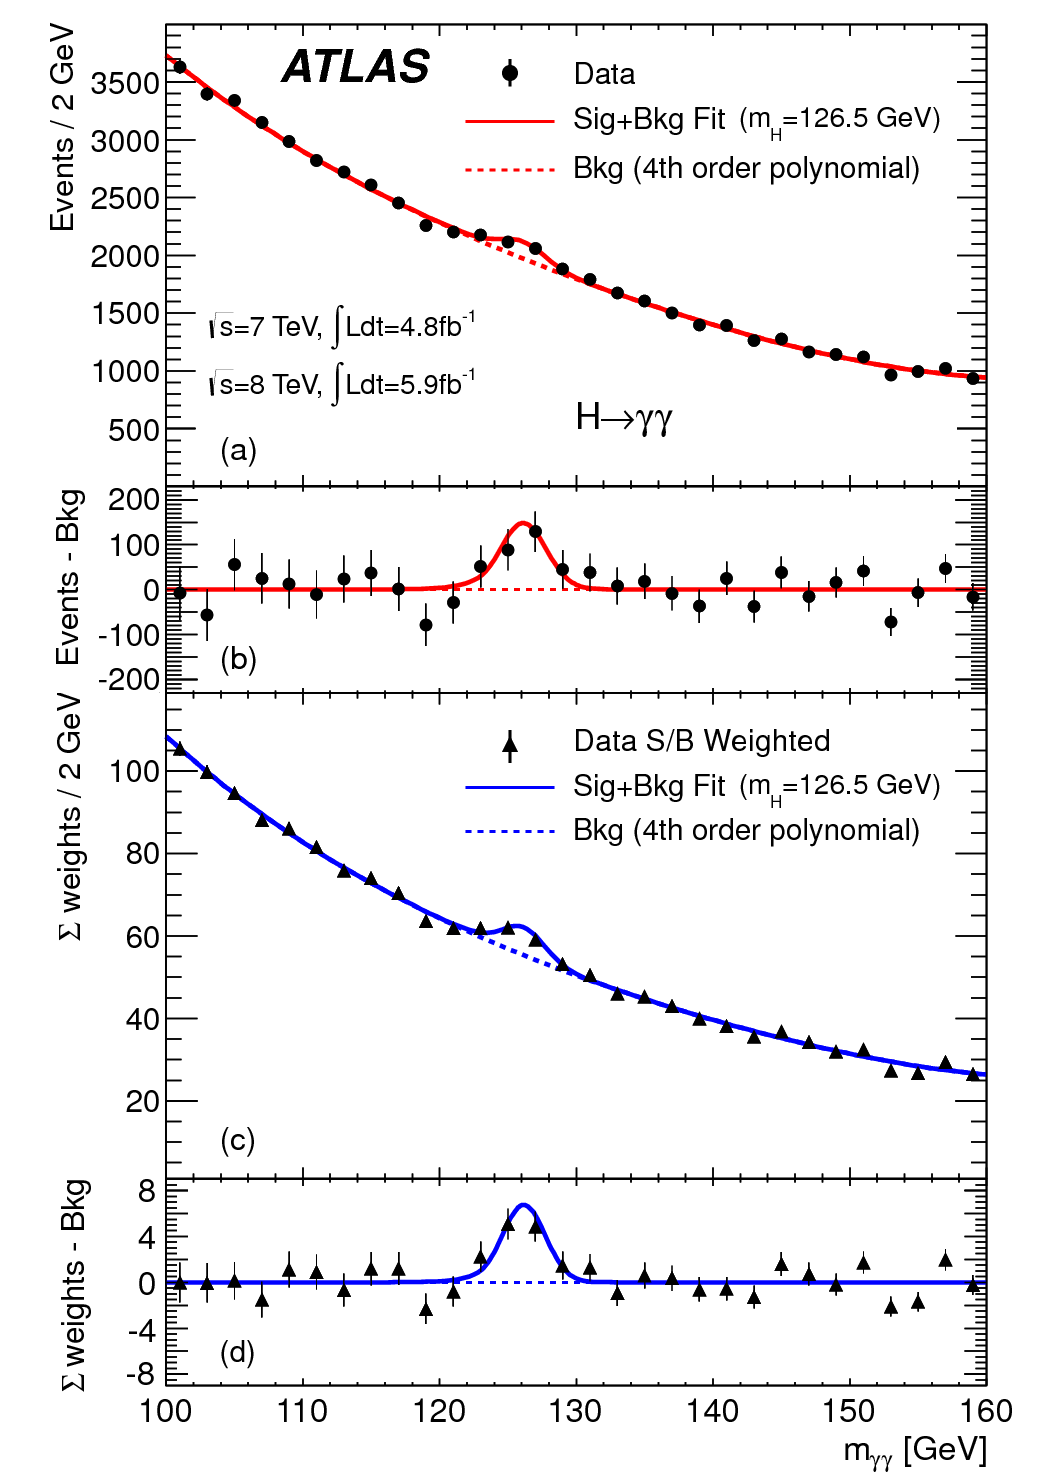
\includegraphics[width=0.6\textwidth]{figures/discovery_mgg}
  \caption{Diphoton mass spectrum in $7$ and $8 \TeV$ data. Panel a) shows the unweighted data distribution superimposed on the background fit, wile panel c) shows the data where each event category is weighted by its signal to background ratio. Panels b) and d) show the respective distributions with background subtracted\cite{Discovery}.}
  \label{fig:disc_mgg}
\end{figure}

\section{$H\to ZZ \to 4\ell$ search}

The $H\to ZZ \to 4\ell$ analysis searches for a Standard Model Higgs boson decaying to two $Z$ bosons, each of which decays to a pair of same flavor, opposite charge isolated leptons. The ultimate discriminating variable is $m_{4\ell}$, or the invariant mass of the four selected leptons. The $\ell$ denotes an $e$ or $\mu$ as with the \HWWfull analysis. Electrons must have $p_{T} > 7 \GeV$ and $|\eta| < 2.47$, while muons must have $\pT > 6 \GeV$ and $|\eta| < 2.7$. There are then additional $\pT$ cuts depending on the relative ranking of the lepton $\pT$, with the leading lepton required to have $\pT > 20 \GeV$, subleading lepton $\pT > 15 \GeV$, and third leading lepton $\pT > 10 \GeV$. 

\subsection{Lepton pair construction}

One of the difficult aspects of this channel is that there are multiple possible same flavor, opposite charge lepton pairs that can be produced out of the four selected leptons. The lepton pair whose mass is closest to $m_Z$ is referred to as the leading pair and its mass is denoted as $m_{12}$, while the other lepton pair's mass is $m_{34}$. Events are required to have $m_{12}$ consistent with a $Z$ mass, or $50 < m_{12} < 106 \GeV$. $m_{34}$ is required to be less than $115 \GeV$. The minimum requirement for $m_{min}$ varies from $17.5 \GeV$ at $m_{4\ell} = 120 \GeV$ to $50 \GeV$ at $m_{4\ell} = 190 \GeV$. 

Four distinct signal regions are constructed depending on the flavors of the final state, additionally separated by the flavor of the leading lepton pair. These are referred to as $4e$, $2e2\mu$, $2\mu2e$, $4\mu$. 

Table~\ref{tab:disc_zz_summary} summarizes the mass resolutions and selection efficiencies for the four signal regions. The mass resolution at $125 \GeV$ is dominated by experimental resolution, ranging from $1.7 \GeV$ to $2.3 \GeV$. 

\begin{table}[h!]
\centering
\captionsetup{justification=centering}

%\begin{tabular*}{0.480\textwidth}{p{0.075\textwidth} p{0.180\textwidth} l}
\hspace{-10pt}
\begin{tabular}{|c|c|c|c|c|}
\hline
Channel & Efficiency & Mass resolution \\ \hline
$4\mu$ & $36\%$ & $1.7 \GeV$ \\ \hline
$2e2\mu$ & $22\%$ & $1.7 \GeV$ \\ \hline
$2\mu2e$ & $22\%$ & $2.2\GeV$ \\ \hline
$4e$ & $20\%$ & $2.3\GeV$ \\ \hline 
\end{tabular}

\caption{
A summary of selection efficiencies and expected resolutions for a $125 \GeV$ Higgs in the $H\to ZZ\to 4\ell$ channel\cite{Discovery}. 
}
\label{tab:disc_zz_summary}
\end{table}

\subsection{Background estimation}

The main backgrounds in the $H\to ZZ \to 4\ell$ search are continuum $ZZ^*$ production, $Z$+ jets production, and $\ttbar$. The $m_{4\ell}$ distribution for background is estimated from simulation. The normalization of the SM $ZZ^*$ background is also taken from MC simulation, while the $Z$+jets and $\ttbar$ normalizations are taken from data-driven methods. The data-driven methods are separated into $\ell\ell+\mu\mu$ and $\ell\ell+ee$ methods. 

In the $\ell\ell+\mu\mu$ case, the control region is defined by relaxing the requirements on the $\mu\mu$ pair to crate a region enriched in background. The $\ttbar$ and $Z$+jets backgrounds are then fit together from the leading mass distribution $m_{12}$. A similar method is used in the $\ell\ell+ee$ case, but there is an additional sorting into categories based on identification criteria for electrons that come from heavy flavor decays or photon conversions. 

\subsection{Results}

Figure~\ref{fig:disc_zz_result} shows the $m_{4\ell}$ spectrum measured in the $7$ and $8 \TeV$ datasets. The total number of events observed in the window between $120$ and $130 \GeV$ is $13$, with $6$ events in the $4\mu$ channel, $2$ events in the $4e$ channel, and $5$ events in the $2e2\mu/2\mu2e$. The best fit $\mu$ value in the combined $7$ and $8 \TeV$ data occurs at $125 \GeV$ and is measured to be $1.2 \pm 0.6$. The observed significance at this mass is $3.6\sigma$, with an expected signficance of $2.7\sigma$. 

\begin{figure}[h!]
  %\vspace{20pt}
  \centering
  \captionsetup{justification=centering}
  %\hspace*{-32pt}
  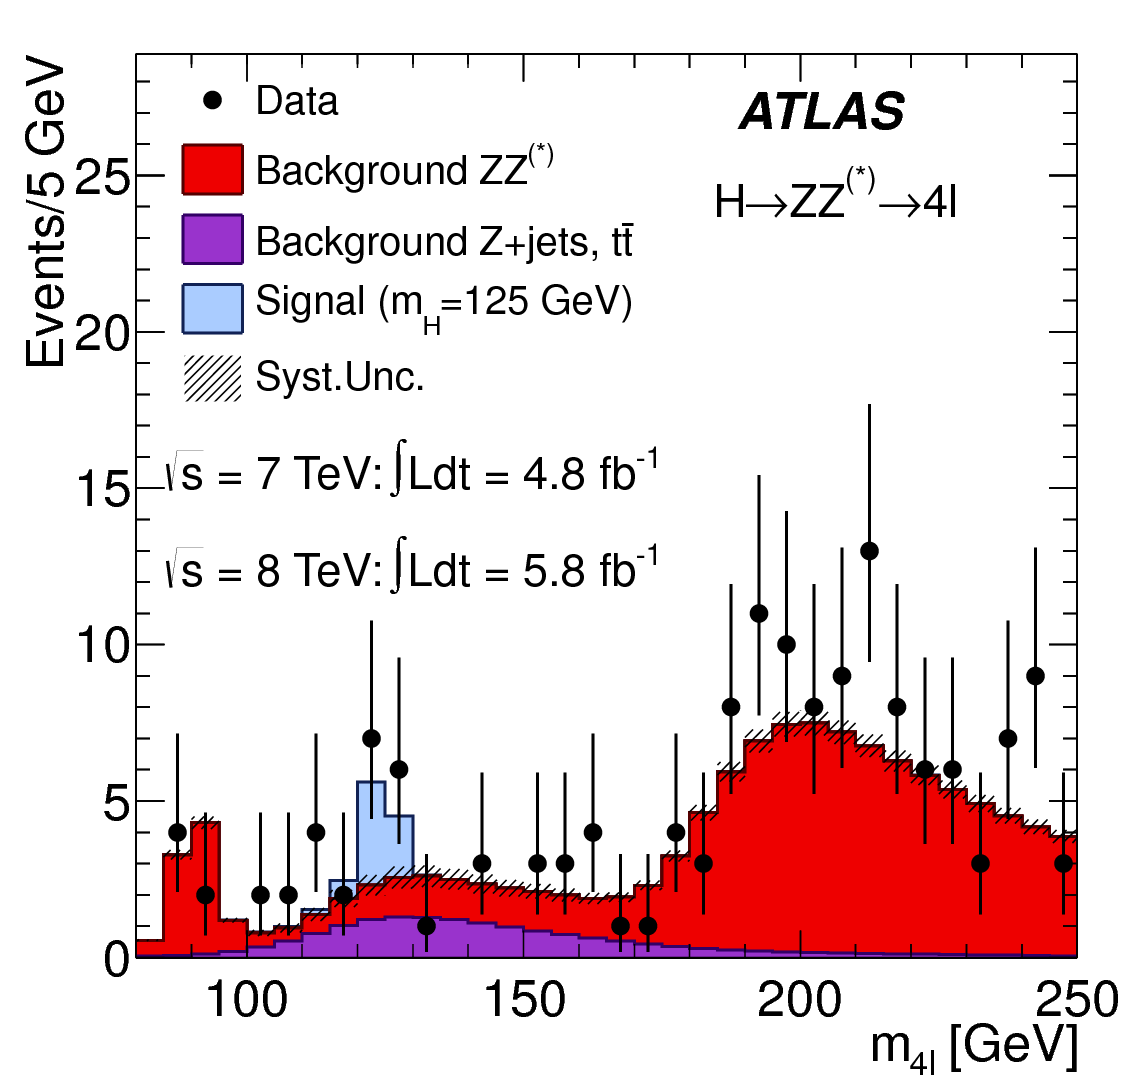
\includegraphics[width=0.6\textwidth]{figures/discovery_m4l}
  \caption{Four lepton invariant mass spectrum ($m_{4\ell}$) in $7$ and $8 \TeV$ data compared to background estimate. A $125 \GeV$ SM Higgs signal is shown in blue\cite{Discovery}.}
  \label{fig:disc_zz_result}
\end{figure}

\section{$H\to WW \to e\nu\mu\nu$ search}

The $H\to WW \to e\nu\mu\nu$ search is unique compared to the $ZZ$ and $\gamma\gamma$ channels. The Higgs mass cannot be fully reconstructed due to the presence of neutrinos in the final state, so the transverse mass $\mT$ is used as the final discriminating variable. Compared to the other channels, there are more backgrounds here as well, as discussed in chapter 3. The same flavor final states are excluded from this search due to high pileup in the $8 \TeV$ dataset. 

\subsection{Event selection}

The analysis requires to opposite charge isolated leptons, with the leading (sub-leading) lepton required to have $\pT > 25 (15) \GeV$. The events are separated into different signal regions depending on which flavor of lepton is leading ($e\mu$ for leading electron, $\mu e$ for leading muon). Strict lepton quality cuts are applied to the sample to reduce backgrounds from fake leptons.

Jets are reconstructed with the anti-$k_{T}$ algorithm with a radius parameter $R = 0.4$. The jets are required to have $\pT > 25 \GeV$ and $|eta| < 4.5$, with jets in the tracking volume required to have a jet vertex fraction of $0.5$ and jets in the forward region required to have $\pT > 30 \GeV$. The analysis is separated into three different signal regions based on jet multiplicity: $\Njet = 0, 1, \geq 2$. 

To indicate the presence of neutrinos in the event, a requirement of $\METrel > 25 \GeV$ is made. This requirement significantly reduces the QCD multijet and $\ZDY$ + jets backgrounds. 

Additional selections are applied to require the dilepton topology to correspond to that of a SM Higgs. The requirements are presented here - more detailed discussion on the motivation for each requirement is saved for Chapter 5. In all of the jet multiplicity channels, the dilepton system is required to have a small gap in azimuthal angle, $\dphill < 1.8$. Similarly, the $\mll$ is required to be less than $50 \GeV$ in the lower jet multiciplicity channels and less than $80 \GeV$ in the $\Njet \geq 2$ channel.  In the $\Njet = 0$ channel, the magnitude of the dilepton $\pT$, $\pTll$, is required to be greater than $30 \GeV$. 

In the higher jet multiplicity channels ($\Njet \geq 1$), the top background is a more important component and must be reduced. The total transverse momentum $\pTtot$ is thus required to be less than $30 \GeV$. Additionally, the di-$\tau$ invariant mass $m_{\tau\tau}$ (dilepton mass computed under the assumption that the neutrinos from the $\tau$ decay are emitted collinear to the charged leptons) is used to reject $Z\to\tau\tau$ events by requiring $|m_{\tau\tau} - m_{Z}| > 25 \GeV$. These variables are also discussed in more detail in Chapter 5. 

In the $\Njet \geq 2$ channel, requirements are made to isolate the VBF contribution to Higgs production. The kinematics of the two leading jets are used to make these requirements. In particular, the event must have $\dyjj > 3.8$ and $\mjj > 500 \GeV$, along with a veto on having any additional jets with rapidity between the to leading jets. 

\subsection{Background estimation}

The details of the background estimation techniques used in the \HWWfull analysis are discussed in section~\ref{sec:HWWbkg}. As that section refers to a later iteration of the analysis, a general discussion is given here for completeness. The dominant backgrounds are SM $WW$ production and top (both pair and single) production, and these backgrounds have their normalizations estimated from dedicated control regions while their shapes are taken from simulation. The $W$+jets background estimate is taken entirely from data using a control sample with one well reconstructed lepton and one anti-identified lepton. All other backgrounds are taken purely from simulation. 

\subsection{Results}

Figure~\ref{fig:disc_mt} shows the $\mT$ distribution in the $\Njet \leq 1$ channels for $8 \TeV$ data. (No events are observed in data in the $\Njet \geq 2$ channels in this dataset). The excess shown here relatively flat as a function of hypothesized Higgs mass. The combined $7$ and $8\TeV$ data gives an excess with local significance of $2.8\sigma$ with an expected significance of $2.3\sigma$, corresponding to a $\mu$ measurement of $1.3\pm 0.5$. 

\begin{figure}[h!]
  %\vspace{20pt}
  \centering
  \captionsetup{justification=centering}
  %\hspace*{-32pt}
  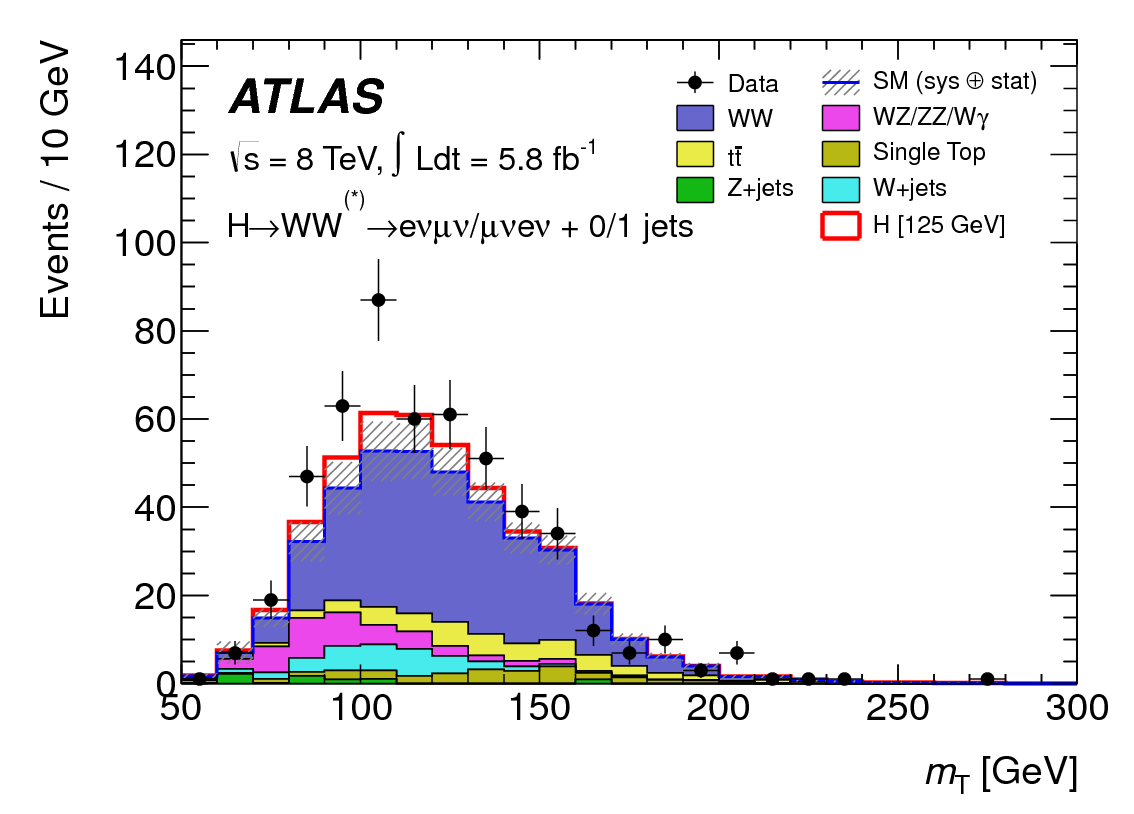
\includegraphics[width=0.6\textwidth]{figures/discovery_mt}
  \caption{$\mT$ distribution in the $H\to WW \to e\nu\mu\nu$ $\Njet \leq 1$ channels for $8 \TeV$ data\cite{Discovery}.}
  \label{fig:disc_mt}
\end{figure}

\section{Combined results}

The statistical interpretation of the combined results is undertaken as described in section~\ref{sec:ww_stats}, with a hypothesis test based on a likelihood ratio parameterized by the Higgs signal strength $\mu$. The null hypothesis corresponds to $\mu = 0$, while the SM Higgs corresponds to $\mu = 1$. 

Table~\ref{tab:discovery_summary} summarizes the properties of the individual channels as well as the significances of the excesses seen. The most significant observed local excess comes from the $\gamma\gamma$ channel. Figure~\ref{fig:disc_p0_comp} shows a comparison of the observed local $p_0$ values as a function of hypothesized mass for the three different search channels. Both the $ZZ^*$ and $\gamma\gamma$ channels ahve very peaked excesses, while the $WW^*$ excess can be seen as very broad because the $\mT$ distribution does not provide detailed information about the true Higgs mass. 

\begin{table}[h!]
\centering
\captionsetup{justification=centering}

%\begin{tabular*}{0.480\textwidth}{p{0.075\textwidth} p{0.180\textwidth} l}
\hspace{-10pt}
\begin{tabular}{|c|c|c|c|c|}
\hline
Channel & Fit var. & Observed $Z_l$ & Expected $Z_l$ & $\hat{\mu}$ \\ \hline
$H\to ZZ^* \to 4\ell$ & $m_{4\ell}$ & $3.6$ & $2.7$ & $1.2 \pm 0.6$ \\ \hline
$H\to\gamma\gamma$ & $m_{\gamma\gamma}$ & $4.5$ & $2.5$ & $1.8 \pm 0.5$ \\ \hline
$H\to WW^* \to e\nu\mu\nu$ & $\mT$ & $2.8$ & $2.3$ & $1.3 \pm 0.5$ \\ \hline
Combined & - & $6.0$ & $4.9$ & $1.4 \pm 0.3$ \\ \hline
\end{tabular}

\caption{
Summary of the expected and observed significance and measured signal strengths in the combined $7$ and $8 \TeV$ datasets for the Higgs discovery analysis\cite{Discovery}. 
}
\label{tab:discovery_summary}
\end{table}

\begin{figure}[h!]
  %\vspace{20pt}
  \centering
  \captionsetup{justification=centering}
  %\hspace*{-32pt}
  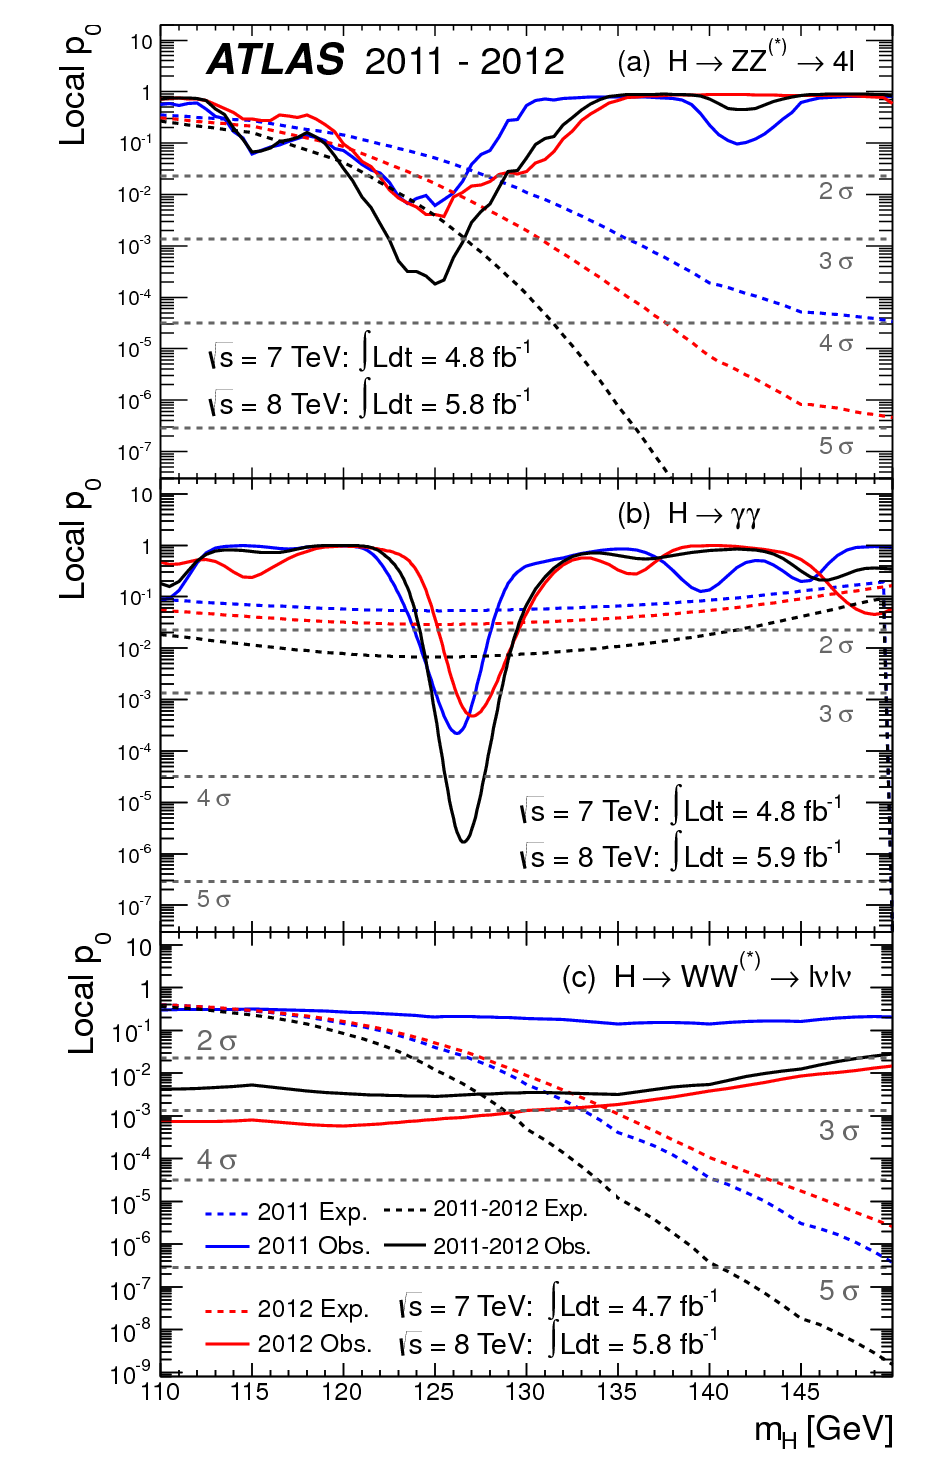
\includegraphics[width=0.6\textwidth]{figures/discovery_p0_comp}
  \caption{Local $p_0$ distribution as a function of hypothesized Higgs mass for the $H\to ZZ^* \to 4\ell$ (a), $H\to\gamma\gamma$ (b), and $H\to WW^*\to \ell\nu\ell\nu$ (c) channels. Dashed curves show expected results, while solid curves show observed. Red curves are from $7 \TeV$ data, blue curves from $8\TeV$, and black curved combined\cite{Discovery}.}
  \label{fig:disc_p0_comp}
\end{figure}

Figure~\ref{fig:discovery_combined} shows the combined exlusion limit, $p_0$, and signal strength. The highest local excess comes at a value of $126.5 \GeV$ and corresponds to a $6.0\sigma$ observed excess. 

\begin{figure}[h!]
  %\vspace{20pt}
  \centering
  \captionsetup{justification=centering}
  %\hspace*{-32pt}
  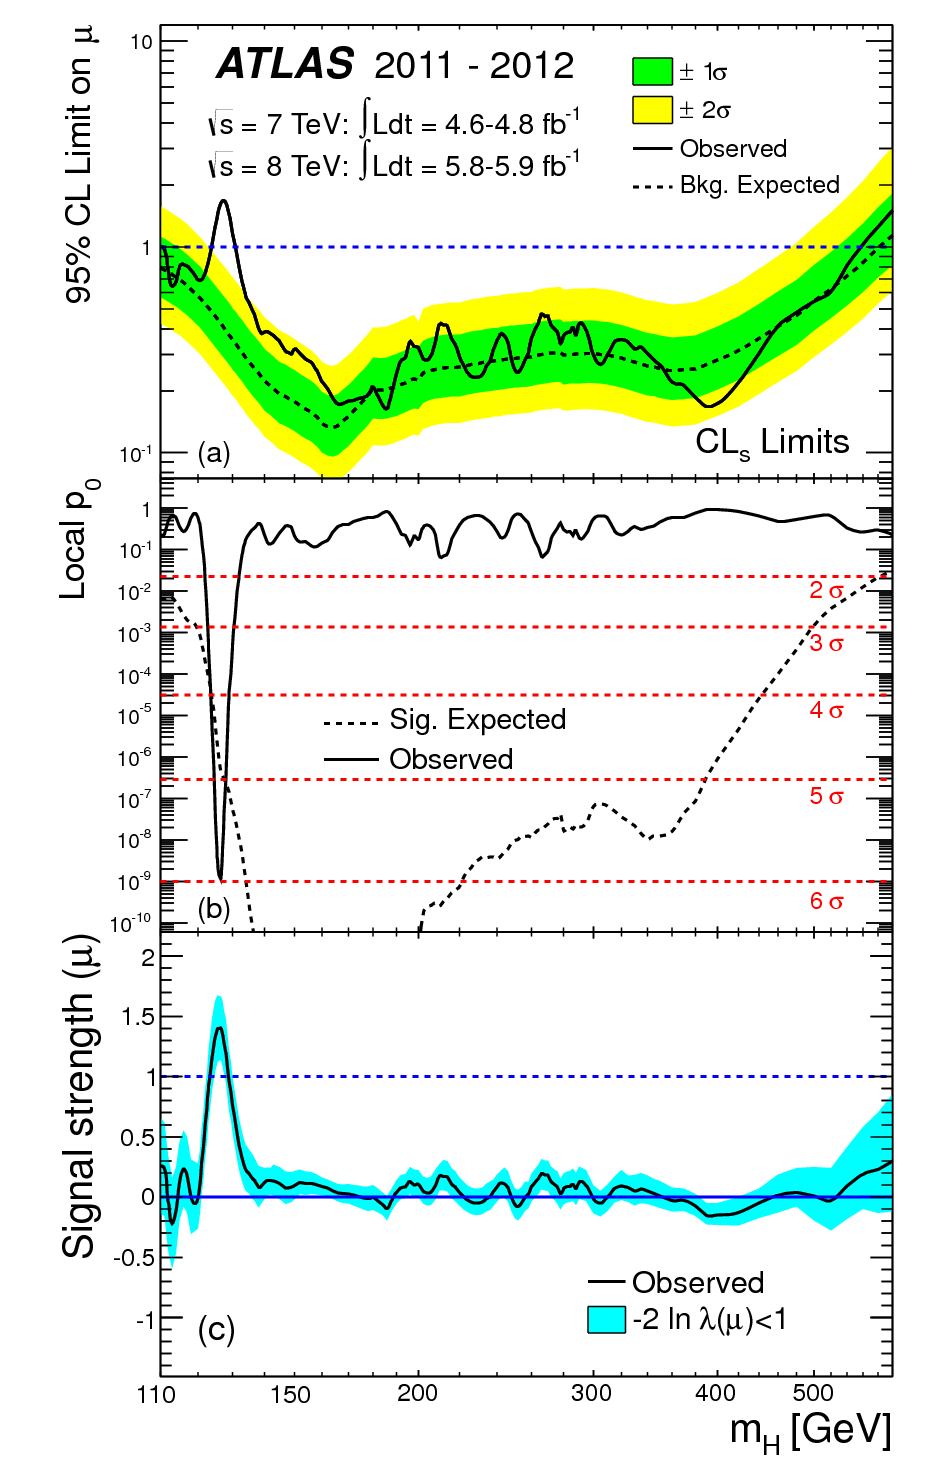
\includegraphics[width=0.6\textwidth]{figures/discovery_combined}
  \caption{Combined 95\% CL limits (a), local $p_0$ values (b), and signal strength measurement (c) as a function of Higgs mass\cite{Discovery}.}
  \label{fig:discovery_combined}
\end{figure}

Figure~\ref{fig:discovery_mu} shows a comparison of the measured signal strengths between the different Higgs search channels. All measured $\mu$ are consistent with unity within their uncertainty, and the combined $\mu$ measurement is $1.4 \pm 0.3$. 

\begin{figure}[h!]
  %\vspace{20pt}
  \centering
  \captionsetup{justification=centering}
  %\hspace*{-32pt}
  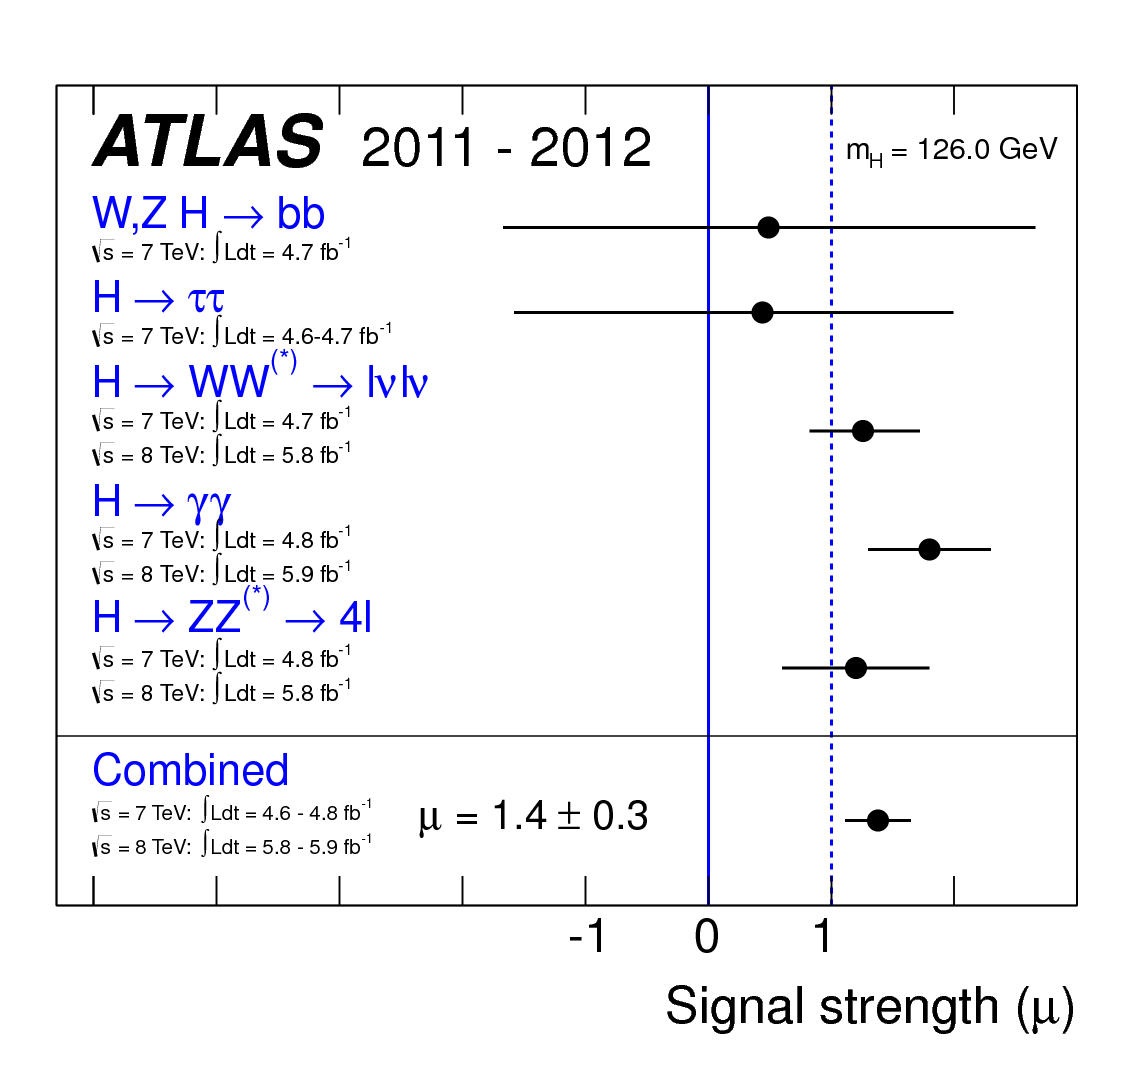
\includegraphics[width=0.6\textwidth]{figures/discovery_mu}
  \caption{Comparison of measured signal strength $\mu$ for a $126 \GeV$ Higgs in the $7$ and $8 \TeV$ datasets\cite{Discovery}.}
  \label{fig:discovery_mu}
\end{figure}

The likelihood can also be computed in a two-dimensional plane of $m_{H}$ and $\mu$, and this is shown in figure~\ref{fig:disc_2d}. The figure shows that while the $\gamma\gamma$ and $ZZ^*$ channels have very good mass resolution, the excess in $WW^*$ covers a broad mass range. The banana shape of the $WW^*$ result is due to the fact that the excess in this channel can either be explained by increasing the signal strength or by changing the mass (and thus the cross section). The two parameters are correlated due to the lack of mass sensitivity in this channel. 

\begin{figure}[h!]
  %\vspace{20pt}
  \centering
  \captionsetup{justification=centering}
  %\hspace*{-32pt}
  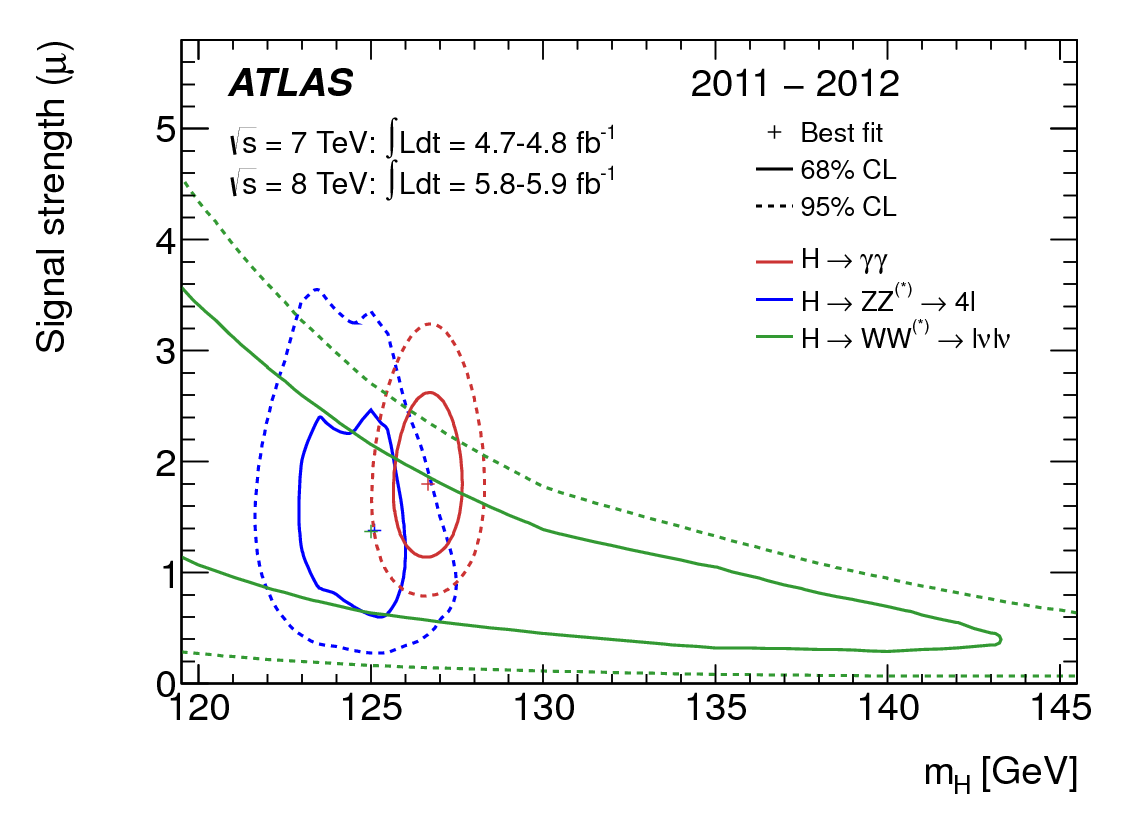
\includegraphics[width=0.6\textwidth]{figures/disc_2d}
  \caption{Two dimensional likelihood as a function of signal strength $\mu$ and Higgs mass $m_H$\cite{Discovery}.}
  \label{fig:disc_2d}
\end{figure}

Because multiple Higgs mass points are searched for, the local significance must be corrected for a look-elsewhere effect to compute a true global significance. The global significance for finding a Higgs anywhere in the mass range of $110 \GeV$ to $600 \GeV$ is $5.1\sigma$. This increases slightly to $5.3\sigma$ if only mass range from $110$ to $150 \GeV$. 

\section{Conclusion}

A search for the production of a Standard Model Higgs boson was conducted in $4.8 \ifb$ collected at $\sqrt{s} = 7 \TeV$ and $5.8 \ifb$ at $\sqrt{s} = 8 \TeV$. A new particle consistent with the Higgs boson was observed, with a mass of $126.5 \GeV$ and a global (local) significance of $5.1 (6.0)\sigma$. This is the first discovery level observation of a particle consistent with the Higgs. 

